\section{Valores y vectores propios}

\subsection{}

{\nologo 
\begin{frame}\frametitle{Valores y vectores propios de una matriz}

\begin{figure}	
	\begin{subfigure}[b]{0.45\textwidth}
		\centering
		\begin{tikzpicture}[thick,scale=0.7, every node/.style={scale=0.6}]%[scale=.8,font=\scriptsize]
		\draw[help lines,white,dotted] (-3,-2) grid (3,2);
		\draw[thick,-latex] (-3,0) -- (3,0) node[below] {\large $x$};
		\draw[thick,-latex] (0,-2) -- (0,2) node[above] {\large $y$};
		%\fill[color=blue] (0,0) circle[radius=2pt];			
		% Vector v
		\draw [line width=0.4mm,color=blue,->] (0,0) -- (1.5,1);
		\fill[color=blue,draw] (1.5,0.8) node[below] {\Large $\mathbf{v} $};	
		% Vector lambda v
		\draw [line width=0.2mm,color=red,->] (0,0) -- (2.5,1.67);
		\fill[color=red,draw] (2.5,1.5) node[below] {\Large $\lambda\mathbf{v} $};	
		\end{tikzpicture}
		\caption{$\lambda>0$}
	\end{subfigure}
	\hfill
	\begin{subfigure}[b]{0.45\textwidth}
		\centering
		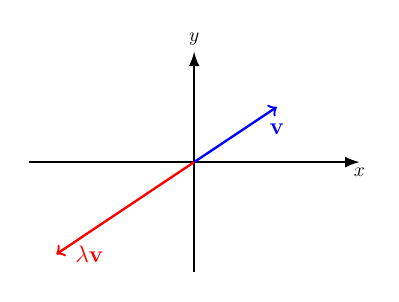
\begin{tikzpicture}[thick,scale=0.7, every node/.style={scale=0.6}]%[scale=.8,font=\scriptsize]
		\draw[help lines,white,dotted] (-3,-2) grid (3,2);
		\draw[thick,-latex] (-3,0) -- (3,0) node[below] {\large $x$};
		\draw[thick,-latex] (0,-2) -- (0,2) node[above] {\large $y$};
		%\fill[color=blue] (0,0) circle[radius=2pt];			
		% Vector v
		\draw [line width=0.3mm,color=blue,->] (0,0) -- (1.5,1);
		\fill[color=blue,draw] (1.5,0.8) node[below] {\Large $\mathbf{v} $};	
		% Vector lambda v
		\draw [line width=0.3mm,color=red,->] (0,0) -- (-2.5,-1.67);
		\fill[color=red,draw] (-1.9,-1.4) node[below] {\Large $\lambda\mathbf{v} $};	
		\end{tikzpicture}
		\caption{$\lambda<0$}
	\end{subfigure}
	%	\caption{Pictures of animals}\label{fig:animals}
\end{figure}

\begin{defi}{\textbf{Definición 1}}\justifying
	\justifying
	Sea $A$ una matriz $n\times n$. Un escalar $\lambda$ (real o complejo) se dice que es un \textbf{\textit{valor propio}}
	de $A$, si existe un vector no nulo $\mathbf{v}$ tal que
	\begin{equation}\label{vp}
		A \mathbf{v} = \lambda \mathbf{v}.
	\end{equation}
	Al vector $\mathbf{v}$ que satisface \eqref{vp} se le denomina \textbf{\textit{vector propio}} de $A$ correspondiente a $\lambda$.
\end{defi}	

\end{frame}
}

%%------------------------------------------------------------------------------------------------------

\subsection{}

{\nologo 
\begin{frame}\frametitle{Valores y vectores propios de una matriz}

\begin{defi}{\textbf{Definición 1}}\justifying
	\justifying
	Sea $A$ una matriz $n\times n$. Un escalar $\lambda$ (real o complejo) se dice que es un \textbf{\textit{valor propio}}
	de $A$, si existe un vector no nulo $\mathbf{v}$ tal que
	\begin{equation}\tag{1}%\label{vp}
	A \mathbf{v} = \lambda \mathbf{v}.
	\end{equation}
	Al vector $\mathbf{v}$ que satisface \eqref{vp} se le denomina \textbf{\textit{vector propio}} de $A$ correspondiente a $\lambda$.
\end{defi}	

\begin{alertblock}{\textbf{Observación 1}}
	\begin{enumerate}[$a$]\justifying
		\item El vector $\mathbf{v}=\mathbf{0}$ no puede ser vector propio de una matriz. \\[2mm]
		\item El escalar $\lambda = 0$ sí puede ser valor propio de una matriz. \\[2mm]
		\item Una matriz puede tener muchos valores propios y repetidos.
		\item A los valores propios de una matriz también se les llama \textbf{\textit{autovalores}}
		o \textbf{\textit{valores característicos}}.
		\item A los vectores propios de una matriz también se les llama \textbf{\textit{autovectores}}
		o \textbf{\textit{vectores característicos}}.
	\end{enumerate}
\end{alertblock}

\end{frame}
}

%%------------------------------------------------------------------------------------------------------

\subsection{}

{\nologo 
\begin{frame}%\frametitle{Valores y vectores propios de una matriz}

\begin{defi}{\textbf{Definición 1}}\justifying
	\justifying
	Sea $A$ una matriz $n\times n$. Un escalar $\lambda$ (real o complejo) se dice que es un \textbf{\textit{valor propio}}
	de $A$, si existe un vector no nulo $\mathbf{v}$ tal que
	\begin{equation}\tag{1}%\label{vp}
	A \mathbf{v} = \lambda \mathbf{v}.
	\end{equation}
	Al vector $\mathbf{v}$ que satisface \eqref{vp} se le denomina \textbf{\textit{vector propio}} de $A$ correspondiente a $\lambda$.
\end{defi}	

\begin{ej}{\textbf{Ejemplo 1}}
	Considere la matriz
	\[
	A =
	\left(
	\begin{array}{rr}
	2 &  0\\[1mm]
	0 & -1
	\end{array}
	\right).
	\]	
	Compruebe que:
	\begin{enumerate}[$a$]
		\item $\mathbf{v}_1=(1,0)$ es un autovector de $A$ correspondiente 
		al autovalor $\lambda_1 = 2$ . \\[2mm]
		\item $\mathbf{v}_2=(0,1)$ es un autovector de $A$ correspondiente 
		al autovalor $\lambda_2 = -1$.
	\end{enumerate}
\end{ej}
\textit{Solución.}

\end{frame}
}

%%------------------------------------------------------------------------------------------------------

\subsection{}

\begin{frame}\frametitle{Valores y vectores propios de una matriz}

%\begin{defi}{\textbf{Definición 1}}\justifying
%	\justifying
%	Sea $A$ una matriz $n\times n$. Un escalar $\lambda$ (real o complejo) se dice que es un \textbf{\textit{valor propio}}
%	de $A$, si existe un vector no nulo $\mathbf{v}$ tal que
%	\begin{equation}\tag{1}%\label{vp}
%	A \mathbf{v} = \lambda \mathbf{v}.
%	\end{equation}
%	Al vector $\mathbf{v}$ que satisface \eqref{vp} se le denomina \textbf{\textit{vector propio}} de $A$ correspondiente a $\lambda$.
%\end{defi}	

\begin{ej}{\textbf{Ejemplo 2}}
	Considere la matriz
	\[
	A =
	\left(
	\begin{array}{rrr}
	1 & -2 & \phantom{-}1 \\[1mm]
	0 &  0 & 0 \\[1mm]
	0 &  1 & 1
	\end{array}
	\right).
	\]	
	Verifique que
	\[
		\mathbf{v}_1=(-3,-1,1) \qquad \text{y} \qquad \mathbf{v}_2=(1,0,0)
	\]
	son vectores propios de $A$ y encuentre sus valores propios correspondientes.
\end{ej}
\textit{Solución.}

\end{frame}

%%------------------------------------------------------------------------------------------------------

\subsection{}

\begin{frame}\frametitle{Valores y vectores propios de una matriz}

%\begin{defi}{\textbf{Definición 1}}\justifying
%	\justifying
%	Sea $A$ una matriz $n\times n$. Un escalar $\lambda$ (real o complejo) se dice que es un \textbf{\textit{valor propio}}
%	de $A$, si existe un vector no nulo $\mathbf{v}$ tal que
%	\begin{equation}\tag{1}%\label{vp}
%	A \mathbf{v} = \lambda \mathbf{v}.
%	\end{equation}
%	Al vector $\mathbf{v}$ que satisface \eqref{vp} se le denomina \textbf{\textit{vector propio}} de $A$ correspondiente a $\lambda$.
%\end{defi}	

\begin{ej}{\textbf{Ejemplo 3}}
	Encuentre los valores propios de la matriz
	\[
	A =
	\left(
	\begin{array}{rr}
	4 & -2 \\[1mm]
	1 &  1
	\end{array}
	\right)
	\]	
	y sus correspondientes vectores propios.
\end{ej}
\textit{Solución.}

\end{frame}

%%------------------------------------------------------------------------------------------------------

\subsection{}

{\nologo 
\begin{frame}\frametitle{Polinomio característico}

\vspace{-2mm}
\begin{defi}{\textbf{Definición 1}}\justifying
	\justifying
	Sea $A$ una matriz $n\times n$. Un escalar $\lambda$ (real o complejo) se dice que es un \textbf{\textit{valor propio}}
	de $A$, si existe un vector no nulo $\mathbf{v}$ tal que
	\begin{equation}\tag{1}%\label{vp}
	A \mathbf{v} = \lambda \mathbf{v}.
	\end{equation}
	Al vector $\mathbf{v}$ que satisface \eqref{vp} se le denomina \textbf{\textit{vector propio}} de $A$ correspondiente a $\lambda$.
\end{defi}	

\vspace{-1mm}
\begin{prop}{\textbf{Propiedad 1}}
	\justifying
	Sea $A$ una matriz $n\times n$. $\lambda$ es un valor propio de $A$ si y sólo si $\det(A-\lambda I)=0$.
\end{prop}	

\vspace{-1mm}
\begin{defi}{\textbf{Definición 2}}\justifying
	\justifying
	Sea $A$ una matriz $n\times n$. El determinante de la matriz $A-\lambda I$ se denota por $p(\lambda)$
	y se denomina el \textbf{\textbf{\textit{polinomio característico}}} de $A$:
	\[
		p(\lambda) = \det(A-\lambda I).
	\]
	La ecuación $p(\lambda) = 0$ se denomina \textbf{\textit{ecuación característica}} de $A$.
\end{defi}	

\end{frame}
}

%%------------------------------------------------------------------------------------------------------

\subsection{}

\begin{frame}%\frametitle{Proceso para encontrar los valores y vectores propios de una matriz}

\begin{ejem}{\textbf{Procedimiento 1}}\justifying
	\justifying
	Sea $A$ una matriz $n\times n$. 
	\begin{enumerate}
		\item Halle el polinomio característico $p(\lambda) = \det(A-\lambda I)$.
		\item Halle las raíces de la ecuación característica $p(\lambda) = \det(A-\lambda I) = 0$.
		\item Resuelva el sistema homogéneo $(A-\lambda_i I) \mathbf{x} = 0$, correspondiente a cada valor propio $\lambda_i$.
	\end{enumerate}
\end{ejem}	

\begin{ej}{\textbf{Ejemplo 4}}
	Encuentre los valores y vectores propios de la matriz
	\[
	A =
	\left(
	\begin{array}{rrr}
	2 & 1 &  0\\[1mm]
	0 & 2 &  0\\[1mm]
	0 & 0 & 2
	\end{array}
	\right)
	\]	
\end{ej}
\textit{Solución.}

\end{frame}

%%------------------------------------------------------------------------------------------------------

\subsection{}

\begin{frame}\frametitle{Propiedades de los valores y vectores propios}
	
	\begin{prop}{\textbf{Propiedad 2}}
		\justifying
		Los valores propios de una matriz triangular son las entradas en su diagonal principal.
	\end{prop}	
		
\end{frame}

%%------------------------------------------------------------------------------------------------------

\subsection{}

\begin{frame}\frametitle{Propiedades de los valores y vectores propios}
	
	\begin{prop}{\textbf{Propiedad 3}}
		\justifying
		Sea $A$ una matriz cuadrada. Entonces $A$ es invertible si y sólo si $0$ \textit{\textbf{no}} es un valor propio de $A$.
	\end{prop}	
	
\end{frame}

%%------------------------------------------------------------------------------------------------------

\subsection{}

\begin{frame}\frametitle{Valores y vectores propios}
	
	\begin{prop}{\textbf{Propiedad 4}}
		\justifying
		Sea $A$ una matriz $n\times n$ con valor propio $\lambda$. Entonces el conjunto 
		\[
		E_{\lambda} = \{ \mathbf{x} \mid A\mathbf{x}=\lambda\mathbf{x} \}
		\]
		es un subespacio.
	\end{prop}		

	
\end{frame}

%%------------------------------------------------------------------------------------------------------

\subsection{}

\begin{frame}\frametitle{Valores y vectores propios}
		
	\begin{defi}{\textbf{Definición 3}}\justifying
		Sea $A$ una matriz $n\times n$ con valor propio $\lambda$. Al subespacio
		\[
		E_{\lambda} = \{ \mathbf{x} \mid A\mathbf{x}=\lambda\mathbf{x} \}
		\]
		se le denomina \textbf{\textit{espacio propio}} o \textbf{\textit{espacio característico}}
		de $\lambda$. A la dimensión de $E_{\lambda}$ se le denomina \textbf{\textit{multiplicidad geométrica}}
		de $\lambda$.
	\end{defi}	

	\begin{alertblock}{\textbf{Observación 2}}
		\[
			E_{\lambda} = \{ \mathbf{x} \mid A\mathbf{x}=\lambda\mathbf{x} \} 
			            = \{ \mathbf{x} \mid (A-\lambda I)\mathbf{x} = \mathbf{0} \}
			            = N_{A-\lambda I}
		\]
	\end{alertblock}
	
\end{frame}

%%------------------------------------------------------------------------------------------------------

\subsection{}

\begin{frame}\frametitle{Valores y vectores propios de una matriz}
	
	\begin{ejem}{\textbf{Procedimiento 1}}\justifying
		\justifying
		Sea $A$ una matriz $n\times n$. 
		\begin{enumerate}
			\item Halle el polinomio característico $p(\lambda) = \det(A-\lambda I)$.
			\item Halle las raíces de la ecuación característica $p(\lambda) = \det(A-\lambda I) = 0$.
			\item Para cada valor propio $\lambda_i$, halle el espacio propio correspondiente $E_{\lambda_i}$.
		\end{enumerate}
	\end{ejem}		
	
\end{frame}

%%------------------------------------------------------------------------------------------------------

\subsection{}

\begin{frame}\frametitle{Valores y vectores propios de una matriz}
		
	\begin{ej}{\textbf{Ejemplo 5}}
		Encuentre los valores y vectores propios de la matriz
		\[
		A =
		\left(
		\begin{array}{rrr}
		1 & 2 & -1\\[1mm]
		1 & 0 &  1\\[1mm]
		4 & -4 & 5
		\end{array}
		\right)
		\]	
	\end{ej}

	\textit{Solución.}
	
\end{frame}

%%------------------------------------------------------------------------------------------------------

\subsection{}

\begin{frame}\frametitle{Valores y vectores propios de una matriz}
	
%	\begin{ejem}{\textbf{Procedimiento 1}}\justifying
%		\justifying
%		Sea $A$ una matriz $n\times n$. 
%		\begin{enumerate}
%			\item Halle el polinomio característico $p(\lambda) = \det(A-\lambda I)$.
%			\item Halle las raíces de la ecuación característica $p(\lambda) = \det(A-\lambda I) = 0$.
%			\item Para cada valor propio $\lambda_i$, halle el espacio propio correspondiente $E_i$.
%		\end{enumerate}
%	\end{ejem}	
	
	\begin{ej}{\textbf{Ejemplo 6}}
		Encuentre los valores y vectores propios de la matriz
		\[
		A =
		\left(
		\begin{array}{rr}
		2 & -1\\[1mm]		
		5 & -2
		\end{array}
		\right)
		\]	
	\end{ej}
	\textit{Solución.}
	
\end{frame}

%%------------------------------------------------------------------------------------------------------

\subsection{}

\begin{frame}\frametitle{Valores y vectores propios de una matriz}	
	
	\begin{prop}{\textbf{Propiedad 5}}
		\justifying
		Sea $A$ una matriz $n\times n$. Si $\lambda_1,\hdots,\lambda_k$ son $k$ valores propios distintos de $A$, entonces los correspondientes
		vectores propios $\mathbf{v}_1,\hdots,\mathbf{v}_k$ son linealmente independientes.
	\end{prop}		
	
\end{frame}

%%------------------------------------------------------------------------------------------------------

\subsection{}

{\nologo 
\begin{frame}\frametitle{Multiplicidad algebraica y geométrica}	
	
	\vspace{-2mm}	
	\begin{alertblock}{\textbf{Observación 3}}
		En el ejemplo 4, la matriz
		\[
		A =
		\left(
		\begin{array}{rrr}
		2 & 1 &  0\\[1mm]
		0 & 2 &  0\\[1mm]
		0 & 0 & 2
		\end{array}
		\right)
		\]	
		tiene polinomio característico $p(\lambda) = -(\lambda-2)^3$ y $\dim E_{\lambda}=2$.
	\end{alertblock}
	
	\begin{defi}{\textbf{Definición 4}}\justifying
		Sea $A$ una matriz cuadrada y sea $\lambda_i$ un valor propio de $A$.
		\begin{enumerate}[$a$]\justifying 
			\item Se dice que $\lambda_i$ es un valor propio de \textbf{multiplicidad algebraica} $k$, si $(\lambda-\lambda_i)^k$ es la mayor potencia que es factor del polinomio característico de $A$.
			\item La \textbf{multiplicidad geométrica} de $\lambda_i$ se define como la dimensión del espacio propio correspondiente a $\lambda_i$, es decir,
			\[
				\text{ multiplicidad geométrica de } \lambda_i = \dim E_{\lambda_i} = \nu(A-\lambda_i I).
			\]
		\end{enumerate}				
	\end{defi}	
	
\end{frame}
}

%%------------------------------------------------------------------------------------------------------

\subsection{}

\begin{frame}\frametitle{Propiedades de los valores y vectores propios}	

\begin{prop}{\textbf{Propiedad 6}}
	\justifying
	Sea $A$ una matriz cuadrada con valor propio $\lambda$. Entonces 
	\[
	\text{multiplicidad geométrica de } \lambda \ \leq \ \text{multiplicidad algebraica de } \lambda.
	\]
\end{prop}	

\begin{prop}{\textbf{Propiedad 7}}
	\justifying
	Sea $A$ una matriz $n\times n$. Entonces 
	\begin{enumerate}[$a$]\justifying
		\item $A$ tiene $n$ vectores propios \textit{linealmente independientes}
		si y solo si la multiplicidad geométrica de todo valor propio de $A$ es igual a la multiplicidad algebraica.
		\item En particular, $A$ tiene $n$ vectores propios \textit{linealmente independientes} si todos sus valores propios son diferentes.
	\end{enumerate}		
\end{prop}	

\end{frame}

%%------------------------------------------------------------------------------------------------------

\subsection{}

\begin{frame}\frametitle{Propiedades de los valores y vectores propios}

\begin{prop}{\textbf{Propiedad 8}}
	\justifying
	Sean $A$ una matriz cuadrada y $\lambda$ un valor propio de $A$, con vector propio correspondiente $\mathbf{x}$.
	Entonces:
	\begin{enumerate}[$a$]\justifying
		\item Para cualquier entero $n>0$, $\lambda^n$ es un valor propio de $A^n$ con vector propio correspondiente
		$\mathbf{x}$.
		\item Si $A$ es invertible, entonces $\frac{1}{\lambda}$ es un valor propio de $A^{-1}$ con vector propio correspondiente 
		$\mathbf{x}$.
		\item Si $A$ es invertible, entonces para cualquier entero $n$, $\lambda^n$ es un valor propio de $A^n$ con vector propio correspondiente
		$\mathbf{x}$.
	\end{enumerate}		
\end{prop}	

\end{frame}

%%------------------------------------------------------------------------------------------------------

\subsection{}

\begin{frame}\frametitle{Propiedades de los valores y vectores propios}
			
	\begin{ej}{\textbf{Ejemplo 7}}\justifying
		La matriz $A$ dada a continuación, tiene valores propios $\lambda_1=-1$ y $\lambda_2=2$, con vectores 
		propios correspondientes $\mathbf{x}_1$ y $\mathbf{x}_2$.
		\[
		A =
		\left(
		\begin{array}{rr}
		0 & 1\\[1mm]		
		2 & 1
		\end{array}
		\right),\quad 
		\mathbf{x}_1 =
		\left(
		\begin{array}{r}
		1\\[1mm]		
		-1
		\end{array}
		\right), \quad 
		\mathbf{x}_2 =
		\left(
		\begin{array}{r}
		1\\[1mm]		
		2
		\end{array}
		\right).
		\]	
		Calcule 
		\[
		\left(
		\begin{array}{rr}
		0 & 1\\[1mm]		
		2 & 1
		\end{array}
		\right)^{10}
		\left(
		\begin{array}{c}
		5\\[1mm]		
		1
		\end{array}
		\right).
		\]
	\end{ej}
	\textit{Solución.}
	
\end{frame}

%%------------------------------------------------------------------------------------------------------

\subsection{}

\begin{frame}\frametitle{Propiedades de los valores y vectores propios}
	
	\begin{prop}{\textbf{Propiedad 9}}
		\justifying
		Suponga que $A$ es una matriz cuadrada que tiene vectores propios $\mathbf{v}_1 , \mathbf{v}_2 ,\hdots,\mathbf{v}_m$, 
		con correspondientes valores propios $\lambda_1,\lambda_2,\hdots,\lambda_m$. Si $\mathbf{x}$ es un vector en 
		$\r^n$ tal que
		\[
			\mathbf{x} = c_1\mathbf{v}_1 + c_2\mathbf{v}_2 + \cdots + c_m\mathbf{v}_m,
		\]
		entonces para cualquier entero $k$, 
		\[
			A^k\mathbf{x} = c_1{\lambda_1}^k\mathbf{v}_1 + c_2{\lambda_2}^k\mathbf{v}_2 + \cdots + c_m{\lambda_m}^k\mathbf{v}_m.
		\]
	\end{prop}	
	
\end{frame}
